\setlength{\columnsep}{3pt}
\begin{flushleft}
	
	\begin{itemize}
		\item Function is a group of related statements that perform a specific task.
		\item Avoids repetition and makes code reusable. 
		\item Types of functions:
		\begin{itemize}
			\item \textbf{Built-in} functions - Functions that are built into Python.
			\item \textbf{User-defined} functions - Functions defined by the users themselves.
		\end{itemize}
		
		\bigskip
		\item Function working:
		\begin{figure}[h!]
			\centering
			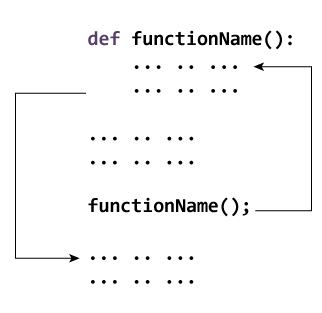
\includegraphics[scale=0.8]{content/chapter6/images/function.png}
		\end{figure}
		
		\begin{tcolorbox}[breakable,notitle,boxrule=1pt,colback=pink,colframe=pink]
			\color{black}
			\fontdimen2\font=8pt
			Syntax: 
			\newline
			def function\_name(parameters):
			 \newline
			\hphantom{} \hphantom{} """docstring"""
			\newline
			\hphantom{} \hphantom{} statement(s)
			\fontdimen2\font=4pt
		\end{tcolorbox}			
		
		\item Explaination:
		\begin{itemize}
			\item Parameters (arguments) through which we pass values to a function. They are
			optional.
			\item A colon (:) to mark the end of function header.
			\item Optional documentation string (docstring) to describe what the function does.
		\end{itemize}
		
		
		\newpage
		\item \textbf{Docstring}: The first string after the function header is called the docstring and is short
for documentation string.
		\newline
		Sample Code:
		\begin{tcolorbox}[breakable,notitle,boxrule=-0pt,colback=black,colframe=black]
			\color{green}
			\fontdimen2\font=9pt
			def testing(): \newline
			\hphantom{} \hphantom{} '''This is test function''' \newline
			\hphantom{} \hphantom{} print("Welcome to python batch") \newline
			\newline
			print(testing.\_\_doc\_\_)
			\fontdimen2\font=4pt
		\end{tcolorbox}
		
		Output:
		\begin{tcolorbox}[breakable,notitle,boxrule=-0pt,colback=output,colframe=output]
			\color{black}
			This is test function
			\fontdimen2\font=4pt
		\end{tcolorbox}
		
		
		
	\end{itemize}
	
\end{flushleft}


